\chapter{Implementación}

En este capítulo se va a proceder a desarrollar cada uno de los PMV de cara a cada hito relacionado con 
la implementación, en los primeros hitos se han dedicado a definir la infraestructura y organización del 
proyecto. De manera que los siguientes hitos se irán definiendo uno tras otro, debido a que el enfoque 
interactivo, principio fundamental del desarrollo ágil, no permite una planificación amplia. Por lo que no 
podríamos establecer todos los PMV desde el principio, además, habrá que discutir qué herramientas van a usarse 
para desarrollar o llevar a cabo estos hitos y el porqué de su elección. 

Primeramente, se decidirá en este caso qué herramienta se usará para albergar el proyecto y poder definir los 
hitos, además de permitir un seguimiento del desarrollo mucho más controlado, siguiendo así con el enfoque ágil 
visto en el primer capítulo. Tras ello se irán desarrollando cada PMV siguiendo las mejores prácticas posibles y 
obteniendo un producto de calidad, principios afines de nuevo al enfoque ágil.



\section{M0: Configuración inicial del TFG - Creación del repositorio}


Ya que el desarrollo avanza a base de productos mínimamente viables, lo primero que 
debemos hacer es definir un repositorio en el que definir estos hitos. Por ello es la primera herramienta
que vamos a elegir. Teniendo en cuenta el uso de git como sistema de control de versiones debido a que es 
la herramienta de control de fuentes más usada genéricamente. 

Teniendo esto presente, buscamos un repositorio basado en git que albergue nuestro proyecto. Además, se busca
una herramienta online y gratuita, por lo que encontramos varias opciones basadas en git que cumplan estas
medidas, como por ejemplo GitHub \footnote{\url{https://github.com/}}, GitLab
\footnote{\url{https://about.gitlab.com/}} y Bitbucket \footnote{\url{https://bitbucket.org/}}, 
plataformas de desarrollo colaborativo que comparten muchas características. 


En general, las versiones gratuitas de estas plataformas son adecuadas para muchos proyectos pequeños y

medianos, al menos las de GitHub y GitLab. Por ello, la elección entre una de estas plataformas depende de 
otros factores, ya que son herramientas muy parecidas, y cualquiera de estas herramientas cumple los criterios
para su elección.


Es por esto que la herramienta elegida será GitHub debido a la familiaridad que se tiene con esta herramienta y 
por ende la comodidad de su uso \footnote{\url{https://github.com/JoseJordanF/Claqueta}}.

Para proseguir con el enfoque sobre la calidad del proyecto, y su control sobre cada cambio en el proyecto, apuntando 
en este caso a la documentación, necesitamos un flujo de trabajo para verificar la ortografía y la gramática de la 
documentación del proyecto. Por ello se hace uso de GitHub Actions una herramienta de integración continua integrada 
en GitHub. Esta herramienta nos guía para crear los flujos de trabajo necesarios, en este caso un verificador 
ortográfico y gramatical, también se aprovechará para crear otro flujo que compile la documentación LaTeX. Debido a 
que es una herramienta con la que se está familiarizado, al igual que con GitHub, es mucho más cómodo su uso. De 
manera que será bastante sencilla la creación de estos flujos de trabajo. Esta podría ser otra razón por la que 
elegir GitHub como repositorio.

Una vez escogido el repositorio y creados los flujos hasta ahora necesarios, nos podemos disponer a dividir la 
implementación del software en hitos. Estos han sido definidos en GitHub y cada uno de ellos contiene un grupo de 
\textit{issues} que sé corresponden con las distintas mejoras que se han ido incorporando al proyecto a lo largo
de su desarrollo.

El uso de herramientas permiten llevar a cabo el proyecto, asegurando su calidad y buenas prácticas 
durante el uso de estas, velando por el enfoque iterativo del proyecto, su adaptabilidad y flexibilidad.
Principios ágiles imprescindibles durante el desarrollo del proyecto, ajustándose estas herramientas a cada
uno de los hitos y adaptándose también a los posibles cambios durante el desarrollo.


Por ello se van a describir las herramientas principales que se van a utilizar para el desarrollo 
del software, en cada uno de los hitos. Describiendo los lenguajes de programación que se usaran, 
lenguajes de consulta y manipulación de datos para API, el modelo de datos a usar, a su vez también 
se mostrarán herramientas que velen por el buen desarrollo en el repositorio y llevar a cabo buenas 
prácticas. El uso de todas estas herramientas será justificado, explicándose así para qué se va a 
utilizar dicha herramienta y porque se ha elegido.

\section{M1: Definición de objetos - Abstracción del dominio del problema}

En este hito \footnote{\url{https://github.com/JoseJordanF/Claqueta/milestone/8}} se conseguirá el 
modelado de los objetos presentes en el problema, para ello se abstraerán 
los conceptos clave y se definirán los objetos de la aplicación. El objetivo es tener una estructura 
clara de los datos a utilizar. La abstracción nos permite identificar las características 
esenciales, eliminando detalles innecesarios. La definición de objetos nos ayudará a comprender sus 
relaciones, atributos y operaciones. Esto establecerá una base sólida para el desarrollo coherente 
de la aplicación.

De esta manera se busca priorizar el desarrollo real, la retroalimentación continua y prácticas como 
el desarrollo impulsado por pruebas \begin{otherlanguage}{english}\textit{(Test Driven Development, TDD)}\end{otherlanguage}  ,y la colaboración cercana. Esto permite una mayor 
agilidad y adaptabilidad en el proceso de desarrollo.

Por ello, buscando un método para definir los objetos de la aplicación, se encuentra una técnica de 
desarrollo de software llamada, \begin{otherlanguage}
{english}``\textit{\textbf{Domain Driven Design}}''\end{otherlanguage}(DDD) \cite{NvDDD} es un enfoque 
de diseño de software que se centra en comprender y modelar el dominio del problema de una aplicación. 
Busca desarrollar un diseño que refleje con precisión las reglas y conceptos del dominio, lo que 
resulta en un sistema más mantenible. Teniendo en cuenta que el DDD y el desarrollo ágil son 
compatibles, ya que su aplicación permite construir aplicaciones que se ajusten mejor a las necesidades 
del cliente y evolucionen de manera flexible a medida que se adquiere un mayor entendimiento del 
dominio. DDD proporciona la base conceptual y un diseño sólido para desarrollar modelos de dominio 
claros y significativos, mientras que el enfoque ágil permite una implementación iterativa, rápida y 
adaptativa.

De esta manera se recurre al uso del \textit{\textbf{modelo de dominio}} representación conceptual de 
las entidades, los conceptos, las reglas, objetos inmutables, como los objetos valor y las 
interacciones dentro del dominio del problema. Es una abstracción del mundo real que captura las 
principales entidades y sus relaciones. Esto ofrece una gran ventaja del DDD, ya que esto ayuda a 
alinear el entendimiento y facilita la comunicación efectiva sobre el problema y su solución. Siendo 
los modelos de dominio una parte central y fundamental del DDD, representando el conocimiento y la 
comprensión profunda del problema que se está abordando. Teniendo esto en cuenta se crea un modelo de 
dominio.

\begin{figure}[h]
    \centering
    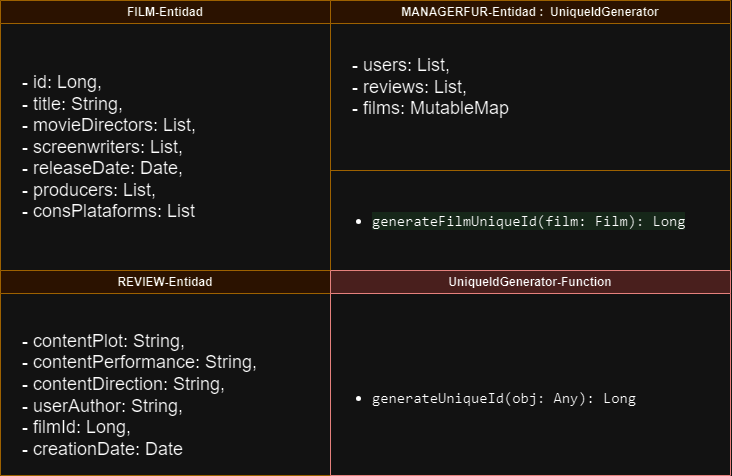
\includegraphics[width=\linewidth]{imagenes/Modelo_Dominio_Claqueta_TFG.drawio.png}
    \caption{Modelo de dominio.}
    \label{fig:diagrama}
\end{figure}



Como base y resumen del modelo de dominio, tendríamos una entidad \begin{otherlanguage}
{english}\textit{\textbf{review }}\end{otherlanguage}haciendo referencia a la reseña, la entidad 
esencial, ya que perseguimos asegurar la calidad de esta. Una reseña de calidad va a ser definida 
comúnmente como una reseña fiable que cumpla las reglas que vimos en el estado del arte. Por lo tanto, 
tendremos atributos generales como el autor de la reseña, un identificador que la relacione con la 
película a la cual está criticando, la fecha de realización de esta crítica y también el 
contenido de la reseña se dividiría para que el usuario hable tanto de la trama general, la 
interpretación y la dirección. Asegurando las reglas vistas en el estado del arte.

Otra entidad importante es la \begin{otherlanguage}{english}\textit{\textbf{film }}\end{otherlanguage} 
siendo su propuesta mínima un conjunto de atributos que definen el contenido de dicha película como los 
directores, los guionistas, la fecha de estreno, las productoras y las plataformas en las que se puede 
consumir dicha película. Este conjunto de atributos es indispensable para la recomendación de dicho 
contenido, siendo cada uno puntos en común que buscar en otras películas para sus recomendaciones 
personalizadas según su contenido. Evidentemente, también necesitamos el título de la película y un 
identificador, ya que el resto de atributos puede coincidir y no identificar de manera única a la 
película.

Por último, tenemos una entidad que se encarga de gestionar tanto películas, como reseñas, como 
usuarios. Además, implementa la interfaz que nos permitirá generar el identificador único para cada 
película.

\subsection{Lenguaje de programación}

Una de las principales herramientas para el desarrollo de software es el lenguaje de programación, un 
lenguaje que sea afín a las necesidades del proyecto. Siendo así un necesario un lenguaje para modelar 
los objetos descritos en este capítulo, en el primer hito. Pero debemos tener en cuenta que se pretende 
que el desarrollo del modelado de los objetos pueda ser reutilizable, de fácil acceso e intentando 
ahorrar recursos. Por ello, para la aplicación es posible crear una API propia, como las que se 
mencionaron en el capítulo del estado del arte. Ya que es muy atractivo que los algoritmos y el modelo 
de datos pueda ser consumido por otros a través de una API

Por ahora deberíamos encontrar un lenguaje que sea flexible y que se adapte a nuestras necesidades. Con 
lo que buscamos un lenguaje de propósito general, lo cual nos permitirá crear diversos proyectos. 
Siendo estos más sencillos de implementar en unos lenguajes que en otros. Podríamos pensar en lenguajes 
como Java, Groovy, Scala o Kotlin. Siendo todos ejecutados en la máquina virtual de java (JVM), siendo 
Java, el veterano, es robusto y multiplataforma, pero su sintaxis puede ser un tanto prolija. Kotlin, 
por su parte, destaca por ser moderno, conciso y compatible con Java, además de ofrecer avanzadas 
características de seguridad. Aunque Groovy simplifica la sintaxis, su velocidad de ejecución más lenta 
podría ser un inconveniente. Scala, con un enfoque en la programación funcional, es expresivo, pero 
puede presentar una curva de aprendizaje más pronunciada. En conclusión, Kotlin emerge como la elección 
óptima en la JVM debido a su curva de aprendizaje suave, su amplia gama de bibliotecas y su excepcional 
interoperabilidad con Java, presentando una combinación equilibrada de simplicidad y funcionalidades 
avanzadas. Siendo bastante atractivo la posibilidad de hacer aplicaciones móviles nativas, punto a 
tratar cuando concluyamos que tipo de aplicación vamos a desarrollar.

\subsection{Persistencia de datos}

La persistencia de datos es primordial para realizar cualquier lógica de negocio. Necesitamos tanto 
datos del usuario como las entidades que representan los objetos con los que interactúan estos 
usuarios. Para ello necesitamos una base de datos, en Kotlin poseemos una gran variedad de opciones. Por 
ejemplo, opciones sencillas de usar y generalmente rápidas como las bases de datos clave-valor, como Firebase 
Database, Redis, Cassandra y LevelDB, ofrecen soluciones para una amplia gama de aplicaciones. Firebase 
Database es ideal para aplicaciones web y móviles que necesitan sincronización en tiempo real. Redis 
sobresale en almacenamiento en memoria y caché, permitiendo la manipulación de varios tipos de datos y 
brindando una rápida recuperación. Cassandra se destaca en la escalabilidad horizontal y la alta 
disponibilidad, adecuada para grandes volúmenes de datos. LevelDB ofrece un almacenamiento eficiente en 
disco. Sin embargo, la elección se inclina hacia Redis, gracias a su capacidad para almacenar datos flexibles 
y variables, y a su facilidad para manejar diversos tipos de estructuras de datos como las vistas en modelo 
de dominó. La curva de aprendizaje es baja para Firebase Database, Redis y LevelDB, mientras que Cassandra 
puede requerir una mayor comprensión de conceptos distribuidos y esquemas de datos más complejos.

También nos podemos apoyar en como se nos indica \cite{NosqlDist}, como podríamos elegir una base de datos 
NoSQL, mencionando como las bases de datos clave-valor son excelentes para datos simples y estructuras 
básicas, adaptándose bastante bien estos modelos de datos. Siendo idóneas para almacenar información de 
sesión o datos en caché, convirtiéndose en una opción sólida si buscamos alta disponibilidad, dado su rápido 
acceso a través de claves, y una escalabilidad horizontal.

\subsection{Inyección de dependencias}

La inyección de dependencias es esencial en proyectos de software \cite{DIart}\cite{BenDI} para 
promover la modularidad y la reutilización del código. Permite desacoplar componentes, lo que facilita 
las pruebas unitarias y el mantenimiento. Al separar la creación de objetos de su uso, se logra una 
mayor flexibilidad y extensibilidad del sistema, lo que facilita la incorporación de nuevas 
funcionalidades sin afectar el código existente. En resumen, la inyección de dependencias promueve un 
diseño limpio y eficiente en el desarrollo de software.

En el mundo de Kotlin, existen varias opciones para facilitar la inyección de dependencias en tus 
proyectos. Koin destaca por su simplicidad y se integra de manera natural con aplicaciones Android. 
Dagger 2, una biblioteca de Google, se basa en anotaciones y brinda una inyección de dependencias 
eficiente y segura, ideal para proyectos extensos. Hilt, una extensión de Dagger 2, simplifica la 
inyección de dependencias en aplicaciones Android, lo que la hace atractiva para desarrolladores 
móviles. Ya que no es un proyecto muy extenso, la opción estaría entre Koin y Hilt. Ambas son buenas 
opciones, sin embargo, Koin es conocido por su enfoque sencillo y sintaxis intuitiva, lo que lo hace 
ideal para proyectos pequeños o si buscas una curva de aprendizaje suave. Por estos dos motivos, Koin 
será la opción seleccionada para llevar a cabo la inyección de dependencias.

\subsection{Testing}

Un proyecto con un enfoque ágil está sujeto a pruebas constantemente, algo que estamos apegando en este 
proyecto a los PMVs resultantes de los milestones. Como ya sabemos de esta manera, aseguramos la 
calidad del producto y nos cerciora de que todo funciona como debería. Consiguiendo así productos de 
calidad más robustos minimizando errores.

Como hemos mencionado, Kotlin goza de acceso a un extenso conjunto de librerías y \textit{frameworks}. 
En este conjunto existen varios \textit{frameworks} que nos permiten testear nuestro código.

Una herramienta esencial para fortalecer el proceso de desarrollo, las pruebas de flujo de trabajo con Docker 
\cite{GI_act}. Esta herramienta nos permite llevar a cabo pruebas exhaustivas de los flujos de trabajo de manera 
local antes de su implementación en el entorno remoto, destacándose por su integración efectiva con Docker. La 
característica distintiva de esta herramienta radica en dicha capacidad para generar simulaciones precisas, 
lanzando y evaluando flujos de trabajo en un entorno controlado basado en Docker. Asegurando la funcionalidad y 
consistencia de los flujos de trabajo antes de su inclusión en el entorno remoto, proporcionando la confianza 
necesaria en la calidad del código. Siendo una herramienta clave para garantizar una implementación sin 
contratiempos, mejorando la robustez y la calidad de los flujos de trabajo antes su despliegue.

Para test unitarios del código encontramos varios \textit{frameworks}, por un lado, tenemos 
\textit{Spek}\footnote{\url{https://github.com/spekframework/spek}}. Una herramienta escrita para 
Kotlin diseñado para facilitar la escritura y ejecución de pruebas en proyectos escritos en este 
lenguaje. Permite definir pruebas en un estilo legible similar al lenguaje natural, lo que facilita 
su comprensión tanto para desarrolladores como para no desarrolladores. Por ello, algunos 
desarrolladores lo relacionan con \begin{otherlanguage}
{english}\textit{Behavior-Driven Development}\end{otherlanguage} (BDD), desarrollo guiado por 
comportamiento. Aunque sus creadores ya han mencionado 
\footnote{\url{https://spekframework.github.io/spek/docs/latest/}} que creen que hay una falsa 
distinción en torno al desarrollo guiado por comportamiento (BDD) y desarrollo guiado por pruebas 
(TDD). Por lo que recomiendan que pensemos en Spek como un simple \textit{framework} de 
especificación.

También disponemos de la herramienta por defecto que incorpora cualquier tipo de proyecto Kotlin, 
\textit{JUnit5}. Este es la última versión del \textit{framework} de pruebas unitarias para Java. Posee 
una arquitectura modular que se compone de tres módulos principales: JUnit Platform, JUnit Jupiter y 
JUnit Vintage, el primero es el núcleo de la herramienta, el segundo introduce las anotaciones y 
permite configurar los test, y la última permite la compatibilidad con versiones anteriores de este 
\textit{framework}. Este es el más usado actualmente por los desarrolladores Android 
\footnote{\url{https://www.jetbrains.com/es-es/lp/devecosystem-2022/testing/}} como nos indica 
\textbf{\textit{Jetbrains}}, compañía que ha diseñado Kotlin.

Ambos son buenas herramientas de pruebas. Además, permiten la integración con otras bibliotecas o 
\textit{framework} de pruebas. Pero ambas herramientas necesitan de otras bibliotecas imprescindibles 
en las pruebas, estas permiten simular objetos de una clase para trucar el resultado de ciertas 
funciones que queremos testear. Estos objetos se denominan \textbf{\textit{Mock}}, en Kotlin 
encontramos la librería nativa \textit{mockk}. Con el par de uno de los \textit{frameworks} 
mencionados y esta librería podríamos realizar los test unitarios que necesitemos. Pero principalmente 
si no en su totalidad usaremos Junit5 debido a la cantidad de información y ejemplos de uso, además de 
ser la usada por la mayoría de desarrolladores Android.

Para la parte de testeo de UI tenemos acceso a varias herramientas, pero nos limitaremos a usar el 
\textit{framework} \textbf{\textit{Espresso}}\footnote{\url{https://developer.android.com/training/testing/espresso?hl=es-419}}, una herramienta creada por Google y la más recomendada \cite{UITest}.

Por último, si fuera necesaria una herramienta para testear las operaciones de una API, si es que 
decidimos crearla, para  recuperar, insertar, modificar o eliminar información. Como hemos visto entre 
las herramientas más usadas para las pruebas\footnote{\url{https://www.jetbrains.com/es-es/lp/devecosystem-2022/testing/}} se encuentra \textit{\textbf{Postman}} una página para ayudar a los 
desarrolladores de API. Por ello es la herramienta que usaremos en tal caso para realizar dichas 
pruebas, además es sencilla y cómoda de usar.

\subsection{M2: Lógica de negocio - Operaciones sobre los datos}

En este hito \footnote{\url{https://github.com/JoseJordanF/Claqueta/milestone/3}} se hablará de la 
lógica de negocio, también conocida como reglas de negocio, se refiere a las operaciones y procesos 
fundamentales que definen cómo funciona la aplicación. Determinando como se procesan los datos, se 
realizan cálculos, se toman decisiones y se llevan a cabo las operaciones clave para lograr los 
objetivos de la aplicación. Siempre dependientes de las necesidades y los propósitos de la aplicación. 
Como estas vienen definidos por las \textbf{Historias de Usuario}, vamos a recurrir a ellas para 
determinar las operaciones que se llevaran a cabo con los datos. Aseguraremos la correcta 
implementación de la lógica de negocio, asegurando la coherencia y validez en las operaciones a través 
de los test unitarios. siguiendo como siempre la esencia del desarrollo ágil, debemos asegurar las
buenas prácticas y garantizar la calidad del proyecto, teniendo en cuenta que la lógica de negocio es 
el núcleo esencial que da vida a una aplicación y hace posible su funcionalidad y utilidad. 

Cabe destacar que lo primero que se hará es crear un proyecto Kotlin creado por gradle, un sistema de 
automatización de construcción de código de software por defecto, en este caso en IntelliJ IDEA. Esto 
es imprescindible, ya que para una mayor comodidad en la configuración y el uso de las distintas 
herramientas que nos ofrece Kotlin es necesario la creación de un proyecto.
Cada una de las siguientes secciones representa un conjunto de issues que se han resuelto para obtener 
un PMV.

Por otro lado, necesitaremos un flujo de trabajo que nos permita seguir unas buenas practicas comprobando
la calidad del código escrito en dicho lenguaje. Cada cambio, cada nueva incorporación al código, se debe asegurar su 
calidad, velando por los principios del enfoque ágil, mencionados en el primer capítulo. Para ello se busca un línter 
o analizador estático de código, siendo este una herramienta que revisa el código en busca de posibles 
errores, malas prácticas o incumplimientos de estilo antes de que se ejecute. Este enfoque proactivo no solo 
ayuda a prevenir problemas antes de que afecten el rendimiento o la funcionalidad del software, sino que 
también se alinea perfectamente con los principios ágiles al fomentar la iteración continua y la mejora 
constante del código, promoviendo así un desarrollo más ágil y eficiente. 

Para la creación de este flujo de trabajo necesitamos un linter para Kotlin que compruebe los ficheros con 
extensión de archivo Kotlin(.kt). Y hacer esto cada vez que añadamos un nuevo archivo Kotlin al repositorio 
o modifiquemos alguno ya existente en algún pull request. Para esta tarea es mucho más rentable usar GitHub 
Actions, ya que debido a su amplia comunidad es sencillo encontrar un linter para el lenguaje que prefieras. 
Por otra parte, la creación del flujo es prácticamente instantánea debido a la guía por parte de GitHub y el conocimiento previo que se tenia de estos al haber usado antes dicha herramienta. 
También es una tarea sencilla y poco pesada para que GitHub Actions la lleve a cabo, y no ocasiona gastos 
adicionales.

Por otro lado, necesitaremos un flujo de trabajo que nos permita comprobar la calidad del código escrito en 
dicho lenguaje. Cada cambio, cada nueva incorporación al código, se debe asegurar su calidad, velando por 
los principios del enfoque ágil, mencionados en el primer capítulo. Para ello se busca un línter o 
analizador estático de código, siendo este una herramienta que revisa el código en busca de posibles 
errores, malas prácticas o incumplimientos de estilo antes de que se ejecute. Este enfoque proactivo no solo 
ayuda a prevenir problemas antes de que afecten el rendimiento o la funcionalidad del software, sino que 
también se alinea perfectamente con los principios ágiles al fomentar la iteración continua y la mejora 
constante del código, promoviendo así un desarrollo más ágil y eficiente. 

Para la creación de este flujo de trabajo necesitamos un linter para Kotlin que compruebe los ficheros con 
extensión de archivo Kotlin(.kt). Y hacer esto cada vez que añadamos un nuevo archivo Kotlin al repositorio 
o modifiquemos alguno ya existente en algún pull request. Para esta tarea es mucho más rentable usar GitHub 
Actions, ya que debido a su amplia comunidad es sencillo encontrar un linter para el lenguaje que prefieras. 
Por otra parte, la creación del flujo es prácticamente instantánea debido a la guía por parte de GitHub y el conocimiento previo que se tenia de estos al haber usando antes dicha herramienta. 
También es una tarea sencilla y poco pesada para que GitHub Actions la lleve a cabo, y no ocasiona gastos 
adicionales.

\subsubsection{Identificación y creación de las películas}

Una vez creado el proyecto con nuestros modelos de dominio, estamos listos para comenzar con las 
distintas operaciones sobre los datos. Para empezar nos deberíamos preguntar qué contenido van a 
consumir los usuarios, claramente películas y en sí las reseñas de estas. Por lo tanto, primeramente 
deberíamos diferenciar de manera única cada película. Para ello tenemos el identificador de cada 
película, pero aún no hemos definido como se creara dicho identificador. Para generar este 
identificador podemos optar por múltiples opciones, se podría pensar que usar el título de la película 
o el nombre de alguno de los directores sería buena idea. Pero esto nos lleva a un problema debido a 
que nos encontramos películas que poseen el mismo título y son diferentes, al igual que los directores. 
Incluso por eso se puede llegar a dar la casualidad de que existan dos películas con el mismo título y 
un director en común, siendo estas diferentes. Por lo tanto, no podríamos usar el título y algún 
director, o al menos si solo usamos estos datos. Por lo tanto, esta deja de ser una posibilidad, aun 
así tenemos muchas más opciones, podríamos recurrir a la base de datos para generar un identificador 
único, ya que muchas bases de datos modernas poseen esta función incorporada. Pero no se quiere 
depender de la base de datos para generar estos identificadores, ya que en este punto del proyecto no 
es necesaria la base de datos. De manera que existen otras opciones como GUID una implementación de 
Windows para generar identificadores siguiendo un algoritmo específico, o alguna otra opción como los 
métodos que usan una marca en el tiempo y un identificador para cada nodo en el sistema. La comparación 
entre ambas opciones \cite{compSnowUUID} nos deja que las opciones estilo UUID son valores de 128 bits 
y no tienen un criterio determinado para generar dicho identificador, mientras que los métodos estilo 
snowflake son valores enteros de 64 bits y tienen una forma determinada de generar dicho identificador. 
debido a la facilidad de seguir un algoritmo determinado y que no necesitamos representar demasiados 
datos como para usar 128 bits, se ha decidido usar snowflake \cite{snowF} método creado por Twitter. 
Básicamente, se basa en crear un identificador único representando en decimal un número binario creado 
por bloques, el primero de 41 bits que define los milisegundos pasados desde una marca de tiempo 
determinada, el segundo bloque de 10 bits representa un identificador propio del objeto, en este caso 
se ha decidido fusionar el título de la película y el nombre del primer director para crear un número 
de 10 bits para este bloque. Por último, el bloque final de 12 bits que simplemente represente un 
número de secuencia por si se da la casualidad que se crean varios objetos en el mismo milisegundo y 
con el mismo título y primer director. Dándonos un identificador que cumple con nuestras necesidades de 
sobra.

\subsubsection{Que es el consumo, quién lo consume y como lo lleva a cabo}

Tras resolver este problema para identificar el contenido, podemos pasar a definir como crear ese 
contenido por parte de la entidad que administra todo. Para ello, cada vez que se crea una película, 
además de introducir todos los datos requeridos, se crea su identificador y se añade a la lista de 
películas del proyecto. Ahora bien, para que este contenido pueda ser consumido por los usuarios dichos 
usuarios deben estar creados en el sistema, por tanto, definimos como se crea un usuario y se introduce 
en la lista de usuarios. Esto nos lleva a responder como definimos el consumo y como designamos que un 
usuario ha consumido, en este caso una película. Lo que nos lleva a una interacción por parte del 
usuario para responder a esas preguntas, a primera vista definimos el consumo, la interacción del 
usuario como la creación de reseñas por parte de este. Siendo las películas en las que reseña o en las 
que interactúa con las reseñas de alguna manera, las películas que consume el usuario. Esto es algo que 
se definirá más adelante en la lógica de negocio. 

\subsubsection{Creación de reseñas}

Una vez creadas las películas y los usuarios, necesitamos definir como se crean las reseñas a través de 
los datos necesarios, la relación con la película y el usuario que la ha escrito. Ya que tenemos todo 
lo necesario para la creación de esta reseña. Dando lugar a la reseña en sí misma y a la marca del 
consumo por parte del usuario, tema mencionado justo en la sección anterior. Además de comprobar que no 
exista una reseña de esa película ya escrita por este usuario, ya que cada usuario solo puede escribir 
una reseña por película.

\subsubsection{Recomendación de contenido al usuario}

Definido el consumo como la realización de reseñas es las distintas películas, tomamos esto como marca 
de consumo como se mencionaba en la creación de reseñas. De esta manera conseguimos el consumo del 
usuario, siendo este todas las películas en las que ha reseñado el usuario. Y siendo las películas 
elegidas para recomendar consumo a este. Las recomendaciones se harán a través de los datos comunes de 
estas películas, los directores, las productoras, los guionistas o las plataformas donde se pueden ver 
estas películas. Cualquiera de estos datos se utilizará para recomendar cualquier película que no se 
haya consumido y tenga algún dato en común con el consumo del usuario. De esta manera tendríamos una 
lista de películas recomendadas para el usuario sin repetidos, ya que es posible que varios datos 
coincidan en las mismas películas. Esta lista se refrescará cada vez que el usuario escriba una reseña 
en una nueva película.

Por cada una de estas operaciones se pueden dar varios casos de uso que se han estudiado a través de 
los test unitarios. Comprobando que cada caso de uso se lleva a cabo como se espera y el conjunto de 
ellos también. Para proseguir con las buenas prácticas y asegurar la calidad del proyecto y de su desarrollo, 
debemos seguir los principios vistos en la introducción sobre enfoque ágil, proporcionando una calidad mayor al 
proyecto y obteniendo un mayor control sobre su desarrollo. Es por esto que debemos crear un flujo de trabajo 
que permita la ejecución de los test unitarios cada vez que se realice un cambio en los ficheros Kotlin del 
proyecto. Por lo tanto, es necesario decidir que herramienta de integración continua vamos a usar para ello. 
GitHub Actions puede usarse perfectamente para la creación del flujo, al igual que se usó para el flujo del 
linter, ya que solo necesitamos ejecutar test unitarios simples que pueden ser ejecutados en una máquina virtual 
Ubuntu y en este caso para estar más seguro del correcto funcionamiento de estos, son ejecutados sobre distintas 
versiones de Java.

\section{M3: Servicios esenciales para la aplicación}

En este hito \footnote{\url{https://github.com/JoseJordanF/Claqueta/milestone/9}} se busca dotar a la aplicación de
dos funcionalidades esenciales para esta, siguiendo el problema planteado por el desarrollador 
\footnote{\url{https://github.com/JoseJordanF/Claqueta/issues/125}}. De esta manera, primero se debe buscar una 
herramienta para el primer servicio, que siguiendo lo expuesto por el desarrollador, debe ser una herramienta que 
permita gestionar la configuración de la aplicación; pudiendo obtener lo necesario para el arranque de la aplicación 
y su posterior funcionamiento. Esta herramienta debe ser capaz de cargar esta configuración desde distintas fuentes, 
velando por el arranque de la aplicación, ya que como menciona el desarrollador, estos ficheros pueden ser de 
distintos tipos, luego afiliarse a uno solo podría llevar desembocar en una carga errónea de este y que la 
aplicación no funcionase. Por lo que se ha recurrido a las fuentes más populares en aplicaciones Kotlin 
\cite{popularConfig} como JSON\cite{JsonWiki}, ficheros Java Properties\cite{JProWiki}, YAML\cite{YmlWiki}, 
HOCON\cite{HoconWiki} o ficheros INI\cite{IniWiki}. Esta sería una de las fuentes independientemente del tipo de 
archivo, otra indudable fuente y más habitual, son las variables de entorno, aunque en lenguajes de la JVM como 
Kotlin aparece otra fuente similar a las variables de entorno del sistema; en este caso se trata de las propiedades
del sistema, en sí de la JVM 
\footnote{\url{https://docs.oracle.com/javase/tutorial/essential/environment/sysprop.html}}. Con estas tres fuentes
se puede crear una jerarquía de lectura según las practicas más habituales en los lenguajes de la JVM 
\footnote{\url{https://docs.appdynamics.com/appd/4.5.x/en/application-monitoring/install-app-server-agents/java-agent/administer-the-java-agent}}, 
en este caso en Kotlin, así se seguirá la siguiente jerarquía, la primera fuente 
será las variables de entorno del sistema, si esta falla se recurrirá a las propiedades del sistema 
\cite{SecrectsJavaP} y por último se recurrirá al archivo de configuración.

Para Kotlin existen mucha variedad de bibliotecas para controlar la configuración de la aplicación, pero se busca 
una que permita el máximo número de fuentes vistas antes, e incluso que permita leer variables de entorno y archivos 
dotenv. Se busca principalmente en el repositorio oficial de Maven \footnote{\url{https://mvnrepository.com/}}, ya 
que brinda una gran cantidad de opciones, además de más información relacionada con la popularidad de la biblioteca 
o las vulnerabilidades que estas tienen. Las bibliotecas encontradas serían las siguientes, Apache Commons 
Configuration\footnote{\url{https://commons.apache.org/proper/commons-configuration/}}, Config de 
Lightbend\footnote{\url{https://github.com/lightbend/config}}, Config 
Magic\footnote{\url{https://github.com/brianm/config-magic}}, Config de 
NetworkNT\footnote{\url{https://mvnrepository.com/artifact/com.networknt/config/2.1.33}}, están listadas en orden de
popularidad, la mayoría tiene soporte para leer de distintas extensiones como JSON o YAML, pero pocas pueden leer de
más de una de estas extensiones; sin embargo, Config de Lightbend y  Config de NetworkNT poseen soporte nativo para 
JSON, ficheros Java Properties y JSON, YAML respectivamente. Pero desgraciadamente ninguna de ellas puede leer 
nativamente archivos dotenv, ni variables de entorno, ni propiedades del sistema. Por lo que se ha decidido usar una 
librería creada por el desarrollador\footnote{\url{https://github.com/JoseJordanF/LibraryConfigProject}}, la 
cual encapsula el funcionamiento de tres bibliotecas, una ya se conoce, ya que es una de las mejores opciones 
discutida arriba, Config de Lightbend que cubre JSON, Java Properties y HOCON, dotenv-
java\footnote{\url{https://github.com/cdimascio/dotenv-java}} que cubre las variables de entorno y los archivos 
dotenv y por último snakeyaml \footnote{\url{https://bitbucket.org/snakeyaml/snakeyaml/src/master/}} que cubre los 
archivos YAML. También de forma nativa lee propiedades del sistema y variables de entorno del sistema, de manera que 
dicha librería lee nativamente archivos JSON, Java Properties, YAML, HOCON e incluso dotenv, además encapsula la 
lectura de fuentes indispensables y más habituales, variables de entorno y propiedades del sistema, por ende es la herramienta 
perfecta para la aplicación.

De modo que la implementación de esta funcionalidad constara de una clase \begin{otherlanguage} {english}``\textit{\textbf{Configurator}}''\end{otherlanguage} 
que permita cargar la configuración siguiendo la jerarquía comentada, y en cualquier momento permitir obtener dichos datos a través 
de dicha clase. Se necesita que solo exista una instancia de esta clase, ya que simplemente se cargara la configuración al inicio de 
la aplicación, sin necesidad de más instancias, aportando control estricto sobre la única instancia, ya que la configuración
trata con secretos delicados. A este patrón de diseño se le conoce como patrón singleton \cite{PattSingl}, en Kotlin 
existen algunas formas de conseguir esto \cite{SinglKotlin} en este caso esto se logra marcando el constructor como 
privado, lo que evita la creación de instancias fuera de la propia clase. Además, se utiliza un objeto companion 
para almacenar esta única instancia y proporcionar un punto de acceso global a través de la clase. De esta manera, 
se asegura que cualquier parte del código pueda acceder a la misma instancia de \begin{otherlanguage} {english}``\textit{\textbf{Configurator}}''\end{otherlanguage}, 
garantizando la coherencia de la configuración en toda la aplicación.

Para la segunda funcionalidad esencial, tal como menciona el desarrollador 
\footnote{\url{https://github.com/JoseJordanF/Claqueta/issues/126}}, se necesita una herramienta que permita 
registrar las distintas acciones de la aplicación para controlar el correcto funcionamiento de esta, y sobre todo 
los errores que se puedan dar durante su ejecución. También debe permitir el registro de la actividad de las 
acciones del usuario; dando estos registros por pantalla o en un archivo de registros, o incluso en ambos, con un 
formato descriptivo para una lectura clara del registro. En este caso, Kotlin o los lenguajes de la JVM poseen 
varias opciones populares, destacando del repositorio de Maven el módulo 
SLF4J\footnote{\url{https://www.slf4j.org/}}. Este módulo sirve de fachada o abstracción para distintos marcos de 
registro muy populares en estos lenguajes, como LogBack\footnote{\url{https://logback.qos.ch/documentation.html}}, 
Log4j 2\footnote{\url{https://logging.apache.org/log4j/2.12.x/}} o Apache Commons 
Logging\footnote{\url{https://commons.apache.org/proper/commons-logging/}}, siendo estos los más usados y populares 
dentro de la comunidad tal como nos indica Maven\footnote{\url{https://mvnrepository.com/open-source/logging-frameworks}}. 
De esas tres bibliotecas, LogBack y Log4j 2 cumplen con los requisitos del desarrollador, ya que Apache Commons 
Logging carece de configuración que permita dar un formato específico a los logs o indicar por la salida de estos, 
además es una fachada comúnmente usada para redirigir los mensajes de registro a SLF4J. Por lo tanto, cualquier 
biblioteca entre las dos mencionadas con anterioridad cumpliría con los requisitos, aun así la elección se va a 
decantar por LogBack, ya que es un poco más popular y usada que Log4j 2.

La implementación de esta funcionalidad será como la anterior, ya que también será una clase singleton
\cite{DPatterns} llamada \begin{otherlanguage} {english}``\textit{\textbf{SimpleLogger}}''\end{otherlanguage}, 
en este caso, ya que pueden crearse múltiples implementaciones del logger sin perturbar el código. Siendo una clase 
singleton para tener control sobre la única instancia existente y que sea más eficiente, ya que será más fácil de 
mantener una sola instancia. Esta se encargará de inicializar el objeto responsable de los registros, indicando la 
configuración de la biblioteca, teniendo en cuenta donde se guardaran los logs, como lo harán y en que formato lo 
harán, esto se consigue gracias a una interfaz que permite definir los componentes necesarios en la configuración de 
la biblioteca, los cuales son el \begin{otherlanguage} {english}``\textit{\textbf{appender}}''\end{otherlanguage} y 
el \begin{otherlanguage} {english}``\textit{\textbf{encoder}}''\end{otherlanguage}, el primero es el encargado de 
donde y como guardar los logs, mientras que el segundo indica el formato en el que lo hacen. De esta manera podremos 
hacer distintas implementaciones de estos métodos para disponer de diferentes tipos de logs.

Por otro lado, también se hace uso de una clase LoggerManager la cual se usa para inyectar la implementación de 
logger que se requiera sin perturbar la implementación en el resto del código. Por último se dará como válida esta
implementación si pasa los test unitarios correspondientes, estos permiten comprobar si sé crean los registros en 
distintas operaciones de la aplicación, de manera que se comprueba su creación y si su información es la que se 
espera. Así se demuestra que las clases que usan el logger lo están usando como deberían y se demuestra que la 
implementación del logger funciona.

\section{M4: Optimización del rendimiento y estandarización del manejo de errores}

En este hito se pretende realizar una refactorización basada en algunas historias del 
desarrollador,\footnote{\url{https://github.com/JoseJordanF/Claqueta/issues/132}}
estas aseguran un funcionamiento más óptimo de la aplicación mediante el uso de las mejores prácticas sobre las 
estructuras de datos, disminuyendo el número de operaciones, o haciendo que estas sean más eficientes. También por 
parte del desarrollador \footnote{\url{https://github.com/JoseJordanF/Claqueta/issues/129}} se pretende establecer una 
jerarquía de clase para los posibles errores que puedan ocurrir en la aplicación. De esta manera se obtendrá una 
refactorización del código actual en el que se siguen las mejores prácticas en el manejo de estructuras de datos y el 
manejo de errores, siendo este el PMV obtenido tras la validación de este hito

Para mejorar la eficiencia de la aplicación se ha recurrido al uso o al cambio de estructuras de datos, como por 
ejemplo las reseñas, anteriormente estaban localizadas en una lista de objetos 
\begin{otherlanguage} {english}``\textit{\textbf{Review}}''\end{otherlanguage}, 
pero esto lo hacía tremendamente ineficiente, ya que si se quisiera buscar las reseñas de un usuario o las reseñas 
de una película tenían que localizarse recorriendo la lista. Pero haciendo uso de un diccionario\cite{OaksJava} que 
relaciona un identificador con un grupo de reseñas es eternamente más eficiente. Para ello se han realizado varios 
cambios, los identificadores únicos han llegado también a los usuarios, ya que la forma de añadir un usuario 
comprobando que no existía ya uno con dicho nombre era bastante ineficiente, ya que requería recorrer la lista, por 
lo que se ha decidido usar un conjunto para guardar los usuarios que ahora serán un objeto definido por un ID único 
al igual que las películas y un string el cual representa el nombre de usuario. Así se ha sobrecargado los métodos 
de conjunto\cite{BlochEffective} para considerar dos usuarios iguales si tienen el mismo nombre de usuario, de manera 
que agregar nuevos usuarios es más sencillo y más eficiente a la hora de comprobar si ya existe alguno con el mismo 
nombre de usuario.

Una vez hecho el cambio de los usuarios, al crear una reseña ahora se añade dos entradas a la estructura de datos 
que las contiene, una representa las reseñas realizadas por el usuario y otra las reseñas referentes a una misma 
película. Así se tendría una eficiencia constante al realizar operaciones de búsqueda sobre dicha 
estructura\cite{LaforeData}; también se hace más eficiente la forma de comprobar si un usuario ya ha escrito una 
reseña sobre una película, ya que el conjunto de reseñas afiliado a esa clave del mapa que representa a una película o 
a un usuario, es un conjunto, de modo que también se sobrecargan los métodos del conjunto para designar una reseña 
igual a otra siempre que los identificadores que guarda dicha reseña sean iguales a los de otra. Así se impide la 
adición de reseñas repetidas porque en un conjunto de reseñas referentes a una película o aún usuario no puede haber 
más de una reseña con la misma ID de usuario o la misma ID de película, respectivamente. Estos cambios han supuesto 
que el resto de operaciones puedan modificarse para ser más eficientes.

Por otra parte, se ha introducido una jerarquía de clase para designar los distintos errores que pueden ocurrir
durante la ejecución de la aplicación, siendo perfectamente identificados los datos que los provocaron, a su vez 
también sé muestra el origen, y se usa un mensaje que explicito para la comprensión del error. Su implementación se 
basa en la creación de clases que heredan de clases que manejan excepciones como lo es 
\begin{otherlanguage} {english}``\textit{\textbf{RuntimeException}}''\end{otherlanguage}, 
dependiendo del tipo de error se decidirá en cada momento de qué clase heredar.

Por último se ha decidido crear una interfaz de la clase base \footnote{\url{https://github.com/JoseJordanF/Claqueta/issues/151}}
para facilitar la escalabilidad de la propia clase y la sencilla implementación de subtipos de ella, abogando por el 
principio de sustitución de Liskov visto en los principios SOLID.

Este hito se dará por válido si pasa todos los test unitarios dispuestos hasta ahora.

 